% !TEX root = ../main.tex
%
\chapter{Related Work}
\label{sec:related}

% feedback-appl
Before describing the problem, and later on the experimental setup, we first
\begin{enumerate}
    \item Introduce three common prediction tasks in \acp{gnn}.
    \item Give a general overview of how \acp{gnn} organize and process graph structured data.
    \item We further discuss the relation of messasge passing mechanism to the WL-test, an algorithm for
          inspecting whether two graphs are isomorph.
    \item Give a formal definition and description of two \ac{gnn}
          architectures which will be used in our experiments.
    \item Discuss typical issues which occur in \acp{gnn} and methods for adressing those issues.
\end{enumerate}


\section{Prediction Tasks and Typical Problems}
\label{sec:related:pred}

% Types of prediction tasks (free-by-me) READY
Graphs naturally appear in numerous application domains, ranging from social analysis, bioinformatics to computer vision.
A Graph $G = (V,E)$, where $V = \{v_{1},...,v_{n}\}$ is a set of $N =|V|$ nodes and $E \subseteq V\times V$ a set of edges betwen those nodes. The unique capability of graphs enables capturing the structural relations among data, and thus allows to harvest more insights compared to analyzing data in isolation~\cite{Zhang19}. Graphs therefore can be seen as a general language for describing entities and relationships between those entities.
\Acfp{gnn} then organize graph structured data to tackle various prediction and classification
tasks. Typically, one is interested in one of the following three tasks:
\begin{enumerate}[label=\textbf{\arabic*.}]
    \item \textbf{Link prediction:}
          Predict whether there are missing links between two nodes
          e.g., knowledge graph completion.

    \item \textbf{Vertex classification \& regression:}
          Predict a property of a node e.g., categorize online users/items.

    \item \textbf{Graph classification \& regression:}
          Here, we are interested in classifying or predicting a continuous value for
          the entire graph, e.g., predicting a property of a molecule.
\end{enumerate}

In this work the main focus will be on \ac{nc}, \ac{gc} and \ac{gr} for small- as well as medium-sized graphs.

% Message passing formally
\section{Passing Messages in \Acsp*{gnn}}
\label{sec:related:message}

% Intro to GNNs, State-description (free-by-me) READY
Graphs, by nature, are unstructured. Vertices in graphs have no natural order and can
contain any type of information. In order for machine learning algorithms to be able
to make use of graph structured data, a mechanism is needed to organize them in a
suitable way~\cite{Zhou2020a,Hamilton2017a,Zhang19}.


% Message Passing in general (free-by-me) READY
Message passing is a mechanism, which embeds into every node information about it's neighbourhood ~\cite{Xu2019,Zhou2020a}. This can be done in several ways. One way of classifying a \ac{gnn} is by looking at the underlying message passing machanism. In this paper we will look at a network, where message passing is done via convolutions (\acf{gcn}). We will however ocasionally use the more general term message passing, as the separation is rather blurred and message passing describes a neighborhood aggregation scheme which is seen as a generalisation of other, more specific mechanisms.

Formally, message passing in a \ac{gnn} can be described as using two functions:
AGGREGATE and COMBINE. The expressive and representational power of a \ac{gnn} can
then be determined by looking at the concrete functions and their properties, used to implement
aggregation and combination. AGGREGATE mixes the hidden representation of every node's neighborhood in every iteration. COMBINE then combines the mixed representation togheter with the representation of the node. Each node uses the information from its neighbors to update its embeddings, thus a natural extension is to use the information to increase the receptive field by performing AGGREGATE and COMBINE multiple times.

\begin{align*}
    a_{v}^{k}   & = \mathrm{AGGREGATE}^{(k)}(\{h_{u}^{(k-1)}: u \in \mathcal{N}_{(v)}\}) \\
    h_{v}^{(k)} & = \mathrm{COMBINE}^{(k)}(h_{v}^{(k-1)}, a_{v}^{(k)})
\end{align*}

For graph-level predictions, an additional READOUT- operation is used:
\begin{align*}
    h_{G} =\mathrm{READOUT}(\{h_{v}^{(K)}\ \mid \ v \in G\})
\end{align*}

% Message passing framework and local graph structure (free-by-me) READY
One useful type of information, which the message passing framework should be able to
capture, is the local graph structure. This can be done by choosing functions with
appropriate properties. A more detailed explanation will follow in
\cref{sec:related:architectures}. In spatial \acp{gnn} we make the assumption of the
similarity of neighbor nodes. To exploit this spatial similarity, we perform
composition by stacking multiple layers togheter increasing the receptive field.

% picture of k-hop neighbourhood aggregation (free-by-me) READY
\begin{figure}[ht]
    \centering
    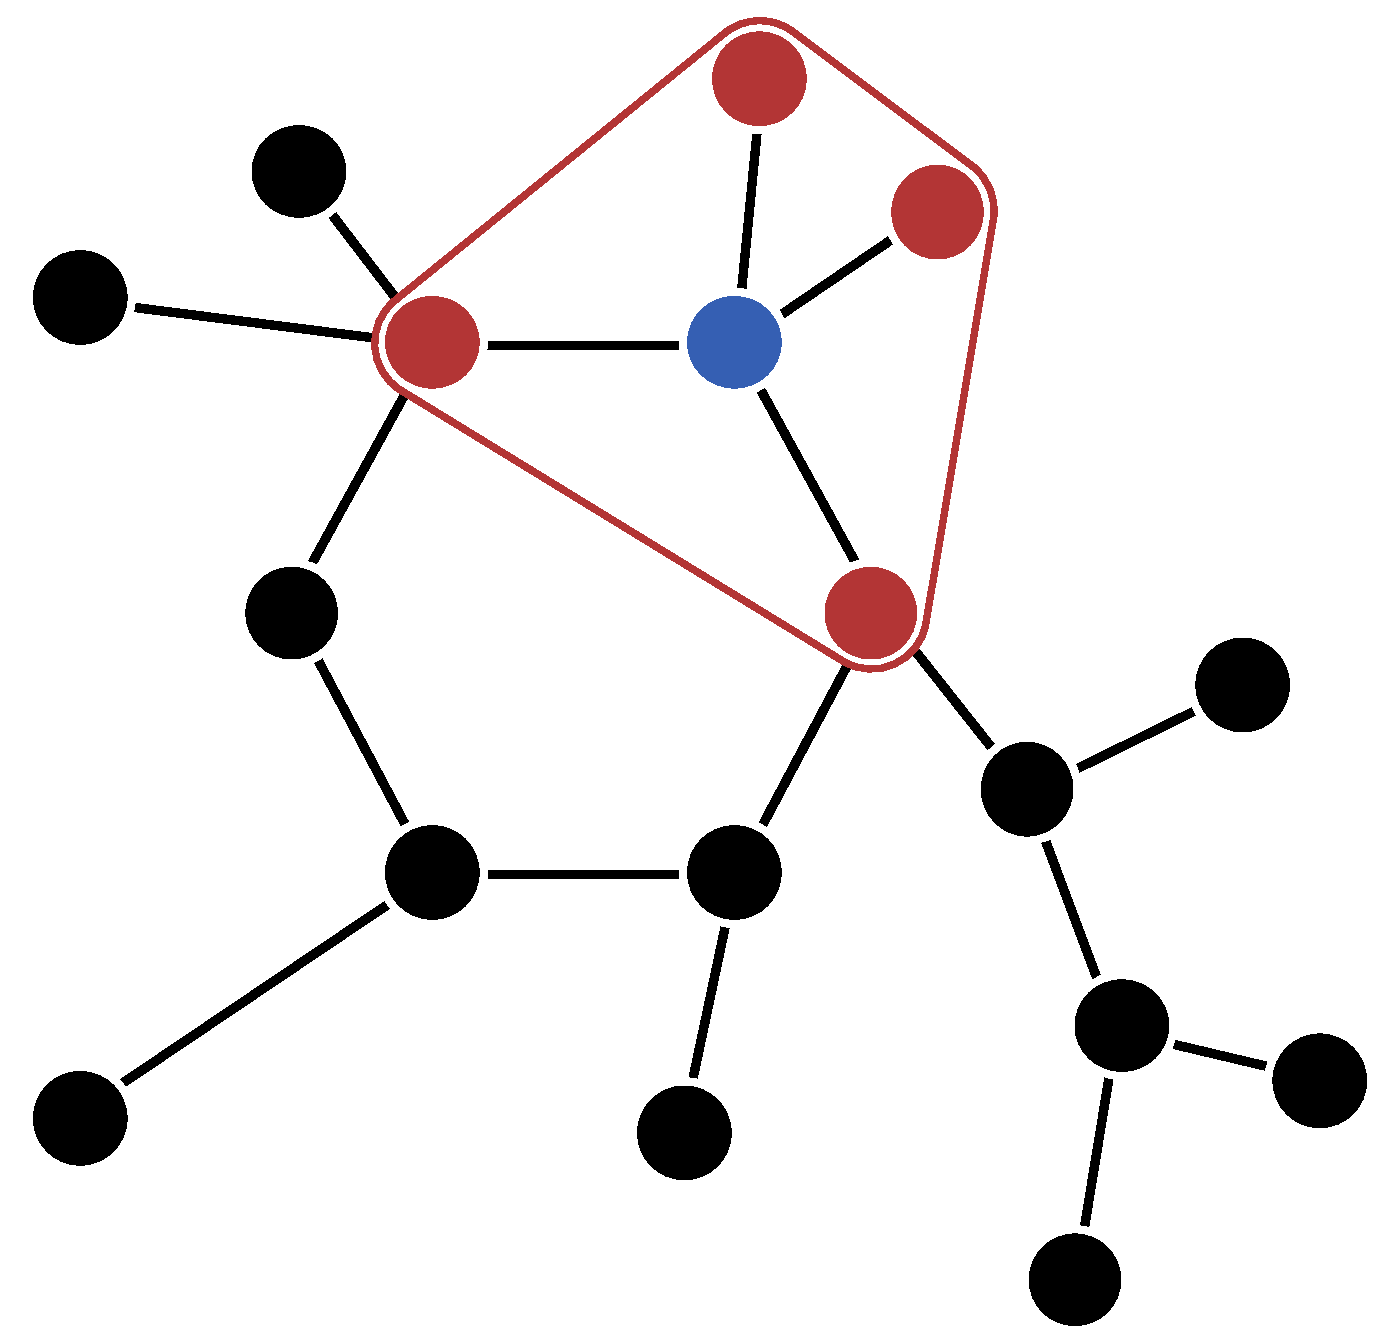
\includegraphics[width=0.35\linewidth]{gfx/related-work/1hop}\hspace{1cm}
    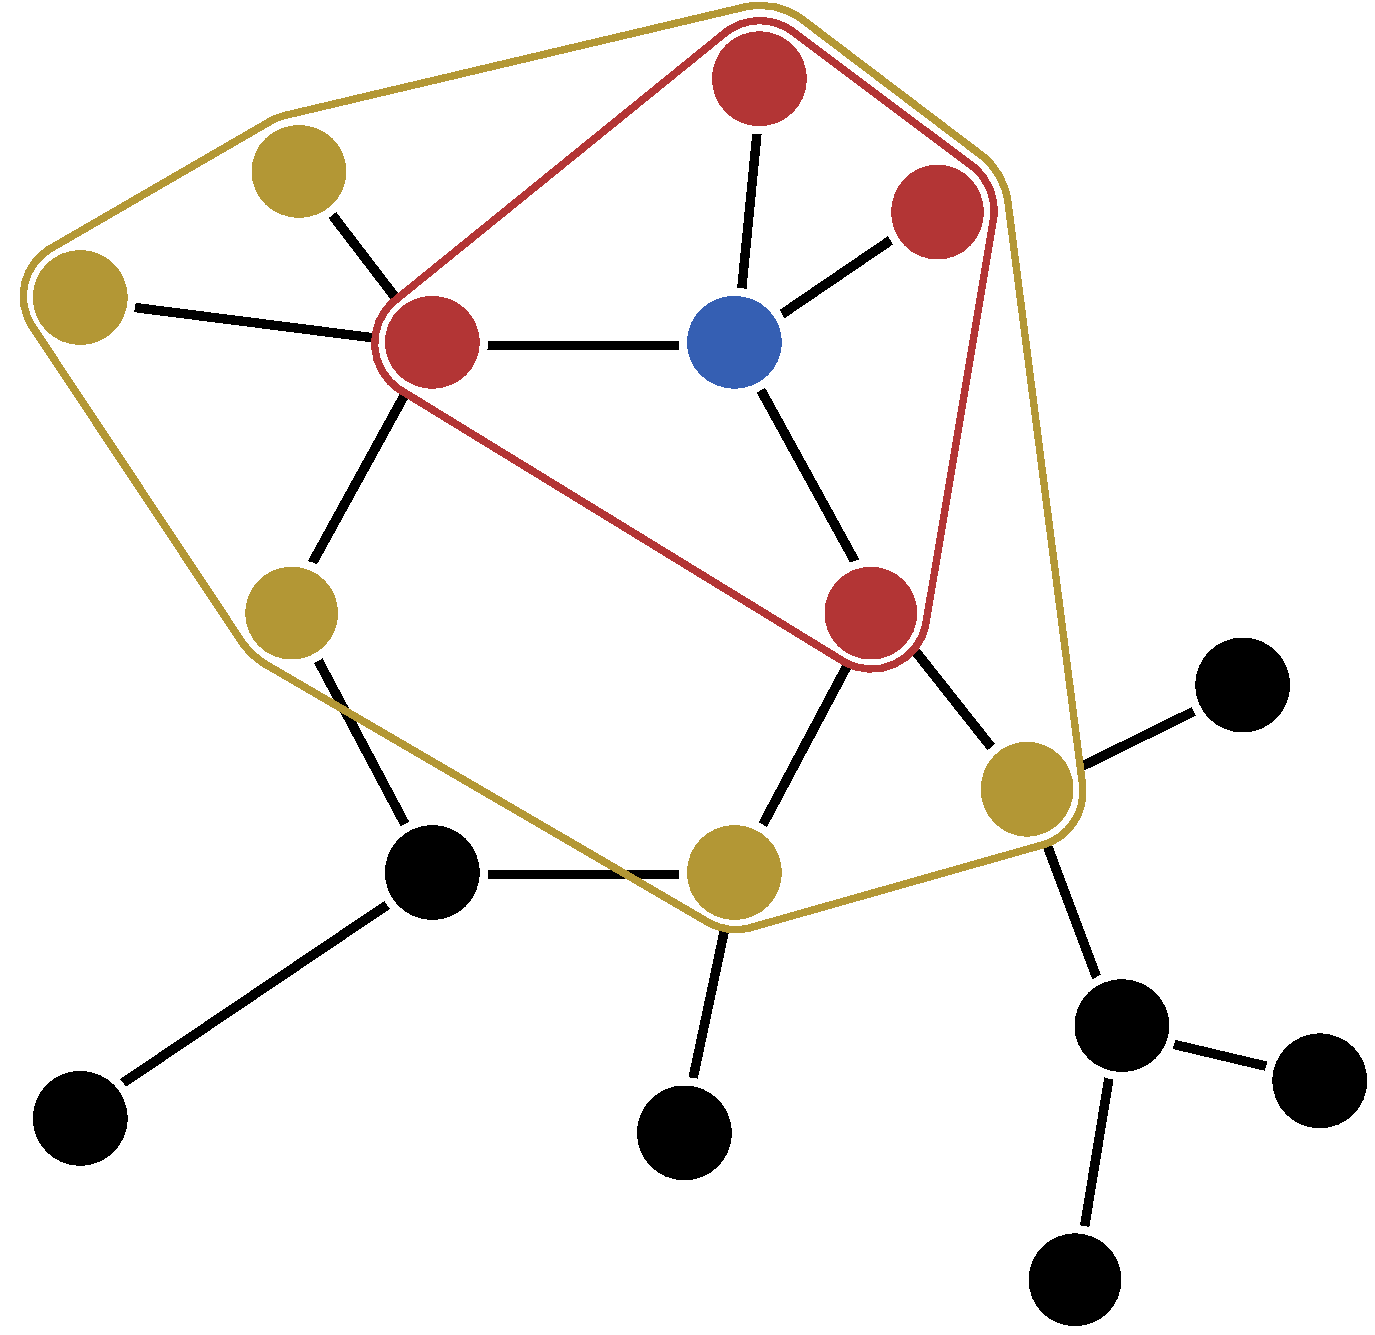
\includegraphics[width=0.35\linewidth]{gfx/related-work/2hop}
    \caption{By performing aggregation $k$-times, we can reach and capture the
        structural information of the $k$-hop neighborhood}\label{fig:related:1hop}
\end{figure}


\subsection{\acl{wl} Graph Colorings}
\label{sec:related:character:wl}
% What is the Weisfeiler Lehman test 
% Definition and relation to neural networks (free-by-me) READY
The Message passing mechanism is closely related to the way the \acf{wl} test ~\cite{Weisfeiler1968,Damke2020,Huang2022} works, an algorithm for deciding if two graphs are isomorphic.
Before describing the algorithm, we introduce notations and preliminaries.\\

% Intro of Notations 
% Graph definition --> Your neighbors are communicating 
Let $G = (V,E, X)$ denote an undirected graph, where $V =\{v_{1},...,v_{n}\}$ is a set of $ N = |V|$ nodes and $E \subseteq V\times V $ a set of edges between those nodes. For simplicity, we represent an edge $\{v,u\} \in E$ by $(v,u) \in E$ or $(u,v)\in E$. $X= [x_{1},...,x_{n}]^{T} \in \mathbb{R}^{n \times d}$ is the node feature matrix, where $n = |V|$ is the number of nodes and $x_{v} \in \mathbb{R}^{d}$ represents the \textit{d}-dimensional feature of node $v$. $\mathcal{N}_{v}= \{u \in V\ \mid \ (v,u) \in E\}$ is the set of neighboring nodes of node $v$. A multiset is denoted
as $\ldblbrace...\rdblbrace$ and formally defined as follows.
% Multiset --> Your neighbors are communicating 
\begin{defn}[Multiset]
    A multiset is a generalization of a set allowing repeating elements. A multiset $\mathcal{X}$ can be formally represented by a 2-tuple as $X = (S_{X}, m_{X})$, where $S_{X}$ is the
    underlying set formed by the distinct elements in the multiset and $m_{X}:S_{X} \rightarrow
        \mathbb{Z}^{+}$ gives the multiplicity (i.e., the number of occurrences) of the elements.
    If the elements in the multiset are generally drawn from a set $X$ (i.e., $S_{X} \subseteq \mathcal{X}$), then $\mathcal{X}$ is the universe of X and we denote it as $X \subseteq \mathcal{X}$ for ease of notation.
\end{defn}
% Isomorphism --> Your neighbors are communicating 
\begin{defn}[Isomorphism]
    Two Graphs $\mathcal{G}= (V,E,X)$ and $\mathcal{H}= (P,F,Y)$ are \textit{isomorphic}, denoted as $\mathcal{G} \simeq \mathcal{H}$, if there exists a \textit{bijective} mapping $g: V \rightarrow P$ such that $x_{v}= y_{g(v)}$, $\forall v \in V$ and $(v,u) \in E$ iff $(g(v),g(u)) \in F$.
\end{defn}
% The 1-WL in its one-dimensional form (free-by-me)
\subsubsection{The 1-dimensional \acs{wl} algorithm (color refinement)}
In the 1-dimensional \ac{wl} algorithm (1-WL), a label, called \emph{color}, $c_{v}^{0}$ is assigned to each vertex of a graph. Then, in every iteration, the colors get updated based on the multiset representation of the neighborhood of the node until convergence. If at some iteration the colorings of the graphs differ, 1-\ac{wl} decides that the graphs are not isomorphic.
\begin{align*}
    c_{v}^{l} \leftarrow \mathrm{HASH}\ (c_{v}^{l-1}, \ldblbrace c_{u}^{l-1}\ \mid \ u \in \mathcal{N}_{v} \rdblbrace)
\end{align*}
\\

Algorithmically, this can be expressed as follows:
% 1-WL algorithm 
\begin{algorithm}[H]
    \caption{1-dim.\ \ac{wl} (color refinement)}
    \begin{algorithmic}[1]
        \Require $G = (V,E,X_{V})$
        \State $c_{v}^{0} \gets \mathit{hash}(X_{v})$ for all $v \in V$
        \Repeat
        \State $c_{v}^{l} \gets \mathit{hash}(c_{v}^{l-1}, \ldblbrace c_{w}^{l-1}: w \in \mathcal N_{G}(v)\rdblbrace)$ forall $v \in V$
        \Until{$(c_{v}^l)_{v \in V} = (c_{v}^{l-1})_{v \in V}$}
        \State \Return $\ldblbrace c_{v}^l : v \in V \rdblbrace$
    \end{algorithmic}
\end{algorithm}

The 1-\ac{wl} is a heuristic method which can efficiently distinguish a broad class of non-isomorphic
graphs~\cite{Babai1979}.
However, there exist some corner cases, where the algorithm fails to classify
simple shapes as non-isomorphic. This is the case for non-isomorphic graphs with the same number of nodes and equivalent sets of node-degrees, as shown in \cref*{fig:related:1-wl-indistinguishable}.

% graphics isomorpc - distinguishable 
\begin{figure}[H]
    \centering
    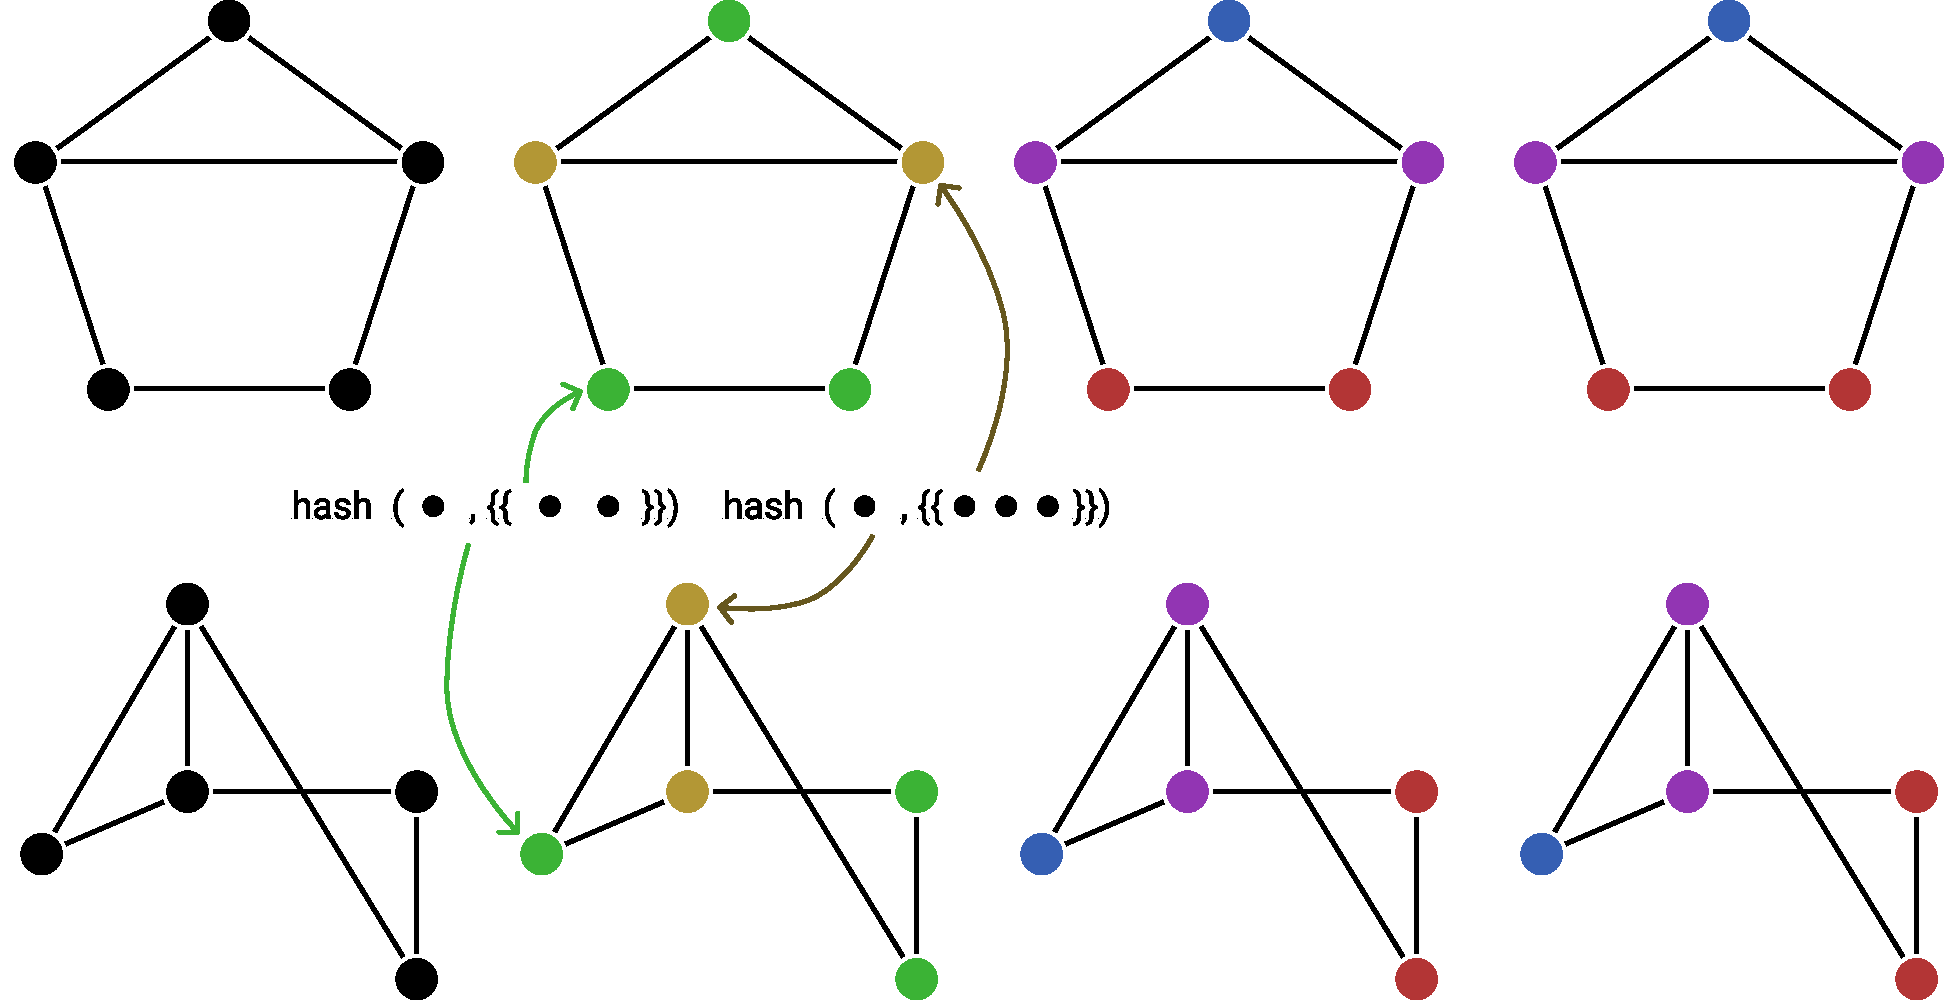
\includegraphics[width= 0.90\linewidth]{gfx/related-work/1wl-isomorph}
    \caption{Two isomorphic graphs. 1-\ac{wl}assigns the same representation to those graphs.}\label{fig:related:1-wl-indistinguishable}
\end{figure}

% graphics isomorpc - indistinguishable 
\begin{figure}[H]
    \centering
    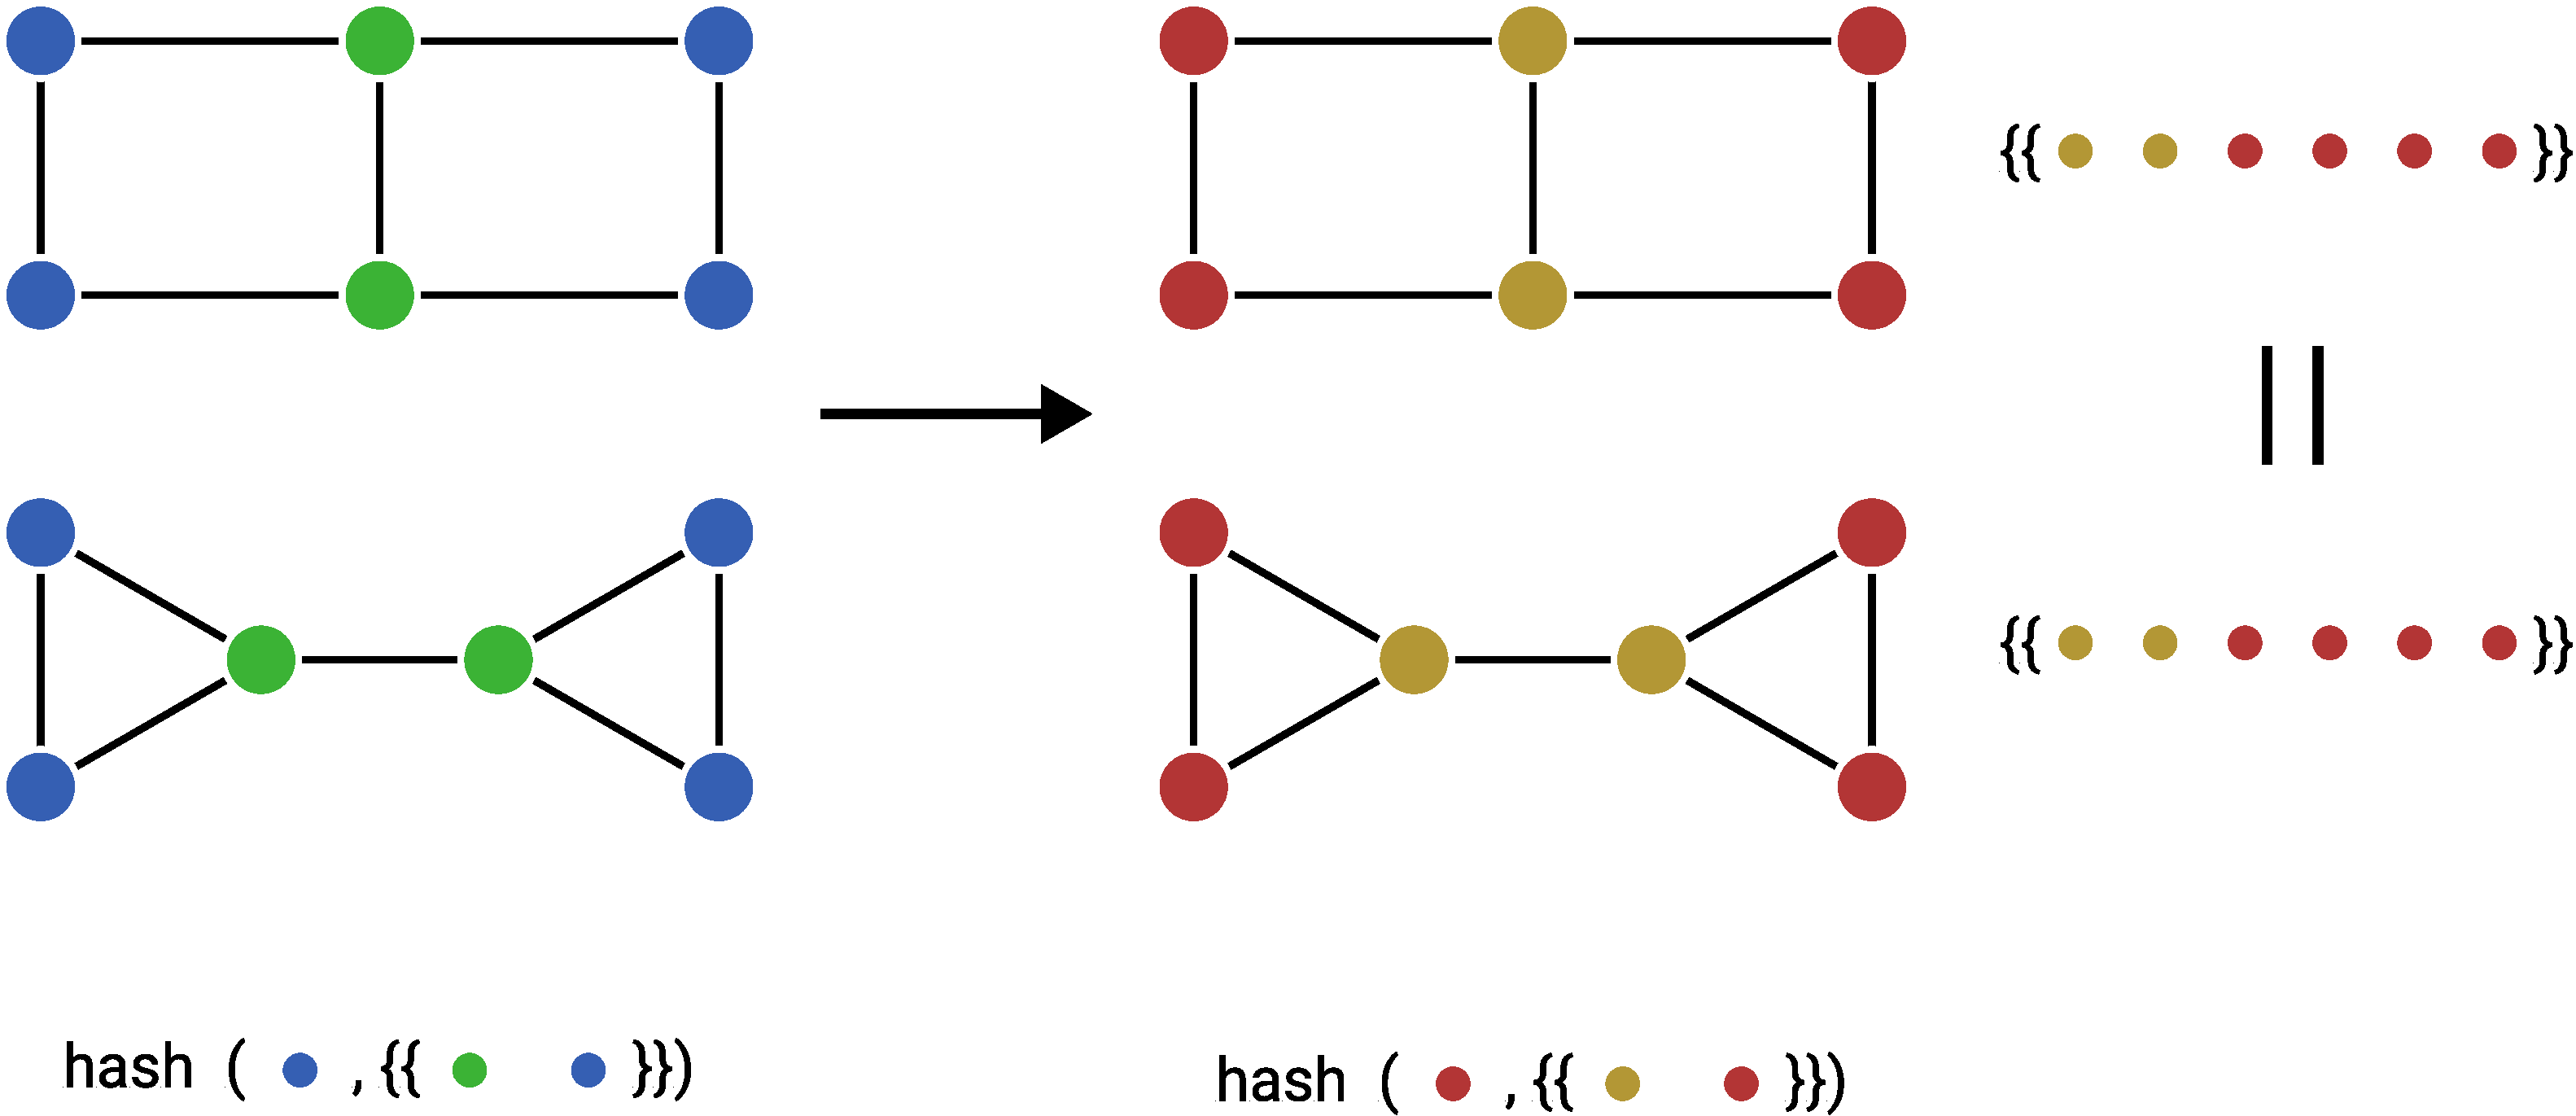
\includegraphics[width= 0.90\linewidth]{gfx/related-work/1wl-indistinguishable}
    \caption{1-\ac{wl} assigned the same labeling to two non-isomorphic graphs~\cite{Liu2022}.}\label{fig:related:1-wl-indistinguishable}
\end{figure}


\subsection{GNN Architectures in this Paper}
\label{sec:related:architectures}

% Intro and motivation of the choice 
% Exploration of important properties 
% Where those networks achieve state of the art results 

% --> Convolutional network --> Image Processing 
% --> GIN, a powerful architecture ---> ecpecially in: 
% Motivation in Conclusion  
In the following section we briefly introduce and
motivate the choice of two types of networks, which we have
chosen to experiementally verify the efficacy of several regularization techniques, which will be discussed in \cref{sec:related:pred:regularization}.

% Explain why these architectures are a promising choice 
Since all \acp{gnn} encorporate message passing in a way, we decided to chose two architectures for our experiments, which are powerful, efficient, scalable and broadly used.
\subsubsection{Graph Convolutional Network (GCN)}
\label{sec:related:architectures:gcn}
% History and Motivation 
\Acf{gcn} was originally proposed by \citet{Kipf2017} to tackle the problem of semi-supervised node classification, where lables are available for a small subset of nodes. \ac{gcn} is a simple, but powerful architecture, that scales linearly in the number of graph
edges and learns hidden layer representations that encode both local graph structure and features of nodes.

% How does it operate formally 
A \ac{gcn} can formally be expressed via the following layer-wise propagation rule:

\begin{align*}
    H^{(l+1)} = \sigma (\tilde{D}^{-\frac{1}{2}}\tilde{A}\tilde{D}^{-\frac{1}{2}} H^{(l)}W^{(l)})
\end{align*}
Where $\tilde{A} = A + I_{N}$ is the adjacency matrix of the undirected graph $\mathcal{G}$
with added self-connections. $I_{N}$ is the identity matrix. $\tilde{D}_{ii} = \sum_{j}\tilde{A}_{ij}$ and $W^{l}$ is a layer-specific trainable weight-matrix. $\sigma(\cdot)$ denotes an activation function, such as $ReLU(\cdot) = max(0, \cdot)$. $ H^{l}\in  \mathbb^{N \times D}$ is the matrix of activations in the
$l^{\mathrm{th}}$ layer; $H^{0}= X$.

% How does it operate intuition --> relation to implementation 
Because we consider every neighbor to be of equal importance and therefore normalization is accomplished
by dividing by the number of neighbours, one can view this operation as performing an element-wise
mean-pooling~\cite{Xu2019}.
\begin{align*}
    h_{v}^{(k)} = \mathrm{ReLU}(\mathrm{W} \cdot\mathrm{MEAN} \{h_{u}^{k-1}\ \mid \ \forall{u} \in \mathcal{N}_{(v)} \cup \{v\}\})
\end{align*}
An application of a two-layer \ac{gcn} is given by:
\begin{align*}
    Z = f(X,A) = \mathrm{softmax} (\hat{A}\ \mathrm{ReLU}(\hat{A}XW^{0})W^{l})
\end{align*}

where $\hat{A} = \tilde{D}^{-\frac{1}{2}}\tilde{A}\tilde{D}^{-\frac{1}{2}}$
is calculated in a preprocessing step. The model uses a single weight matrix per layer and
deals with varying node degrees through an appropriate normalization of the adjacency matrix.
% Experimental results and where it was expecially useful and why 
This model consisting of a 2-layer \ac{gcn} performed well in a series of experimental tasks, including semi-supervised document classification, semi-supervised node classification in citation networks and semi-supervised entity classification in a bipartite graph extracted from a knowledge graph.
The prediction accuracy was evaluated on a set of 1000 examples and additional experiments on deeper models with up to 10 layers have been also provided. Being capable of encoding both graph structure and node features, \ac{gcn} outperformed numerous related methods by a significant margin~\cite{Kipf2017}.

\Acfp{gcn} are widely and successfully used today in many fiels due to their simplicity and scalability.

\subsubsection{Graph Isomorphism Network (GIN)}
\label{sec:related:architectures:gin}
% Overview 
To overcome the lack of expressivity of popular GNN architectures,~\citet{Xu2019} designed a new type of \ac{gnn}, \ac{gin}. They prove that \acp{gin} are strictly more expressive than a variety of previous \ac{gnn} architectures and that they are in fact as powerful as the commonly used 1-dimensional \acf{wl}-test.

% Requirements and condition 
Two requirements must be met for a network to have the same expressive and representational
power as the \ac{wl} isomorphism test:
\begin{enumerate}
    \item The framework must be able to represent the set of feature vectors of a given nodes
          neighbors as a multiset.
    \item Choosing an injective function for the aggregation step. Such a function would never
          map two different neighborhoods to the same representation.
\end{enumerate}
The more discriminative the multiset function is, the more powerful the representational power of the underlying \ac{gnn}.

% Formal definition and explanation 
Formally, a \acf{gin} can be expressed as follows:
\begin{align*}
    h^{(k)}_{v}  = \mathrm{MLP}^{(k)} \left((1 + \epsilon^{(k)}) \cdot h^{(k-1)}_{v} + \smashoperator{\sum_{{u} \in{\mathcal{N}(v)}}} \,h^{(k-1)}_{u}\right) \\
\end{align*}

The choice of such an architecture, is motivated by the necessity to learn two functions with certain properties,
$f$ and $\phi$. This task can be accomplished using a \ac{mlp}.
The following lemma and corollary, proven by~\citet{Xu2019} show the properties and application of the functions:

% Theorem 3 + Lem + Cor 
\begin{thm}
    Let $A: G:\rightarrow \mathbb{R}^{d}$ be a \ac{gnn}. With a sufficient number of \ac{gnn} layers, A maps any grphs $G_{1}$ and $G_{2}$ to different embeddings, the \ac{wl}-test of isomorphism decides as non-isomorphic, to different embeddings if the following conditions hold:
    \begin{enumerate}[label=(\alph*)]
        \item A aggregates and updates node features iteratively with
              \begin{align*}
                  h_{v}^{(k)} = \phi (h_{v}^{(k-1)}, f (\{h_{u}^{(k-1)}\ \mid \ u \in \mathcal{N}_{(v)}\}))
                  \intertext{where the functions f, which operates on multisets and, and $\phi$ are injective.}
              \end{align*}
        \item $A$'s graph-level readout, which operates on the multiset of node features $\{h_{v}^{(k)}\}$, is injective.
    \end{enumerate}
\end{thm}


\begin{lem}
    Assume $\mathcal{X}$ is countable. There exists a function $f:\mathcal{X} \rightarrow \mathbb{R}^n$
    so that $h(X) = \sum_{x \in X}f(x)$ is unique for each multiset $X \subseteq \mathcal{X}$ of bounded size. Moreover, any multiset function g can be decomposed as $g(X) = \phi(\sum_{x \in X}f(x))$
    for some function $\phi$.
\end{lem}

\begin{cor}
    Assume $\mathcal{X}$ is countable. There exists a function $f:\ \mathcal{X} \rightarrow \mathbb{R}^n$
    so that for infinetly many choices of $\epsilon$, including all irrational numbers, $h(c,X) = (1+ \epsilon)\cdot f(c) + \sum_{x \in X}f(x)$
    is unique for each pair (c,X), where $c \in \mathcal{X}$ and $X \subseteq \mathcal{X}$ is a multiset of bounded
    size. Moreover, any function g over such pairs can be decomposed as $g(c,X) = \varphi(1+\epsilon)\dot f(c) +\sum_{x \in X}f(x)$
    for some function $\varphi$.
\end{cor}

\subsubsection{\ac{gin} is as powerful as 1-dimensional\ac{wl}}
% NEW AND UNAPPROVED
\Ac{gin} is a neural network-based approach designed to handle graph data and detect graph isomorphisms. It operates on each vertex and updates its representation based on its own features and the aggregated features of its neighbors. There exists a fundamental similarity between the \ac{gin} and the way the 1-\ac{wl} algorithm works
\subsection{Weaknesses and Obstacles in \acp{gnn}}
\label{sec:related:pred:typical}
% What are the typical problems in GNNs
Because of the way \acp{gnn} operate, they tend to suffer from two main obstacles:
Overfitting and oversmoothing.

% Overfitting description and intuition 
Overfitting hinders the generalization ability of a \acf{nn}, making it perform poorly
on previously unseen data. This occurs expecially when using small datasets, since the model thends to 'memorize' instead of learn the pattern.

% Oversmoothing description and intuition
Oversmoothing is a condition, where the performance and predictive power of a \ac{nn}
does not improve or even gets worse when more layers are added. This happens because
by stacking multiple layers  togheter aggregation is being performed over and over again.
This way, the representation of a node is being smoothed, i.e., mixed with features of
very distant, possibly unrelated nodes. Oversmoothing is a problem mainly for node classification tasks. There is a trade-off between the expressiveness of the model (capturing graph structure by applying multiple layers) and oversmoothing, which leads
to a model where nodes have the same representation, because they all converge to indistinguishable vectors~\cite{Zhou2020,Hasanzadeh2020}.%
\footnote{In spatial \acp{gnn} we make the assumption of relatedness by proximity.}

% Why is this happening?
A closer examination of underlying causes of oversmoothing was conducted by \citet{Chen2020}, who suggested, that not message passing itself, but the type of interacting nodes cause this issue.
For \acf{nc} tasks, intra-class communication (interaction between two nodes sharing the same class) is useful (signal), whereas inter-class communication (the communication between two nodes sharing different lables) is considered harmful, because it brings interference noise into the feature-representations by mixing unrelated features and therefore making unrelated nodes more similar to each other. Because of that, the the quality of shared information is essential and should therefore be considered as a benchmark for improvement.


\subsection{Regularization Techniques}
\label{sec:related:pred:regularization}

% What is Ragularization generally? 
\citet{Kukacka2017} define regularization as any supplementary technique that aims at making the model generalize better, i.e., produce better results on the test set, which can include various properties of the loss function, the loss optimization algorithm, or other techniques.

% Classification of reg.t -> stochastic regularization 
One subgroup of regularization is via data, where the training set $\mathcal{D}$ is
transformed into a new set $\mathcal{D}_{R}$ using some stochastic parameter
$\pi$, which can be used in various ways, including to manipulate the feature space,
create a new, augmented dataset or to change e.g, thin out the hidden layers of
the \ac{nn}.

An example of such a transformation is corruption of inputs by Gaussian noise.
\begin{align*}
    \tau_{0}(x) = x + \theta, \theta \backsim \mathcal{N}(0, \Sigma)
\end{align*}

% Stochastic regularization techniques, data augmentation
In this work we focus on stochastic regularization techniques, which perform
data augmentation in one way or another and whose main benefits lie in the alleviation
of overfitting and oversmoothing \cite{Hasanzadeh2020}.\
We will use the following notation: \

\begin{center}
    \begin{tabular}{ll}
        \toprule
        \textbf{Notation}                                                            & \textbf{Description}                                     \\
        \midrule
        $H^{(l)}= [h_{0}^{(l)},\dots h_{n}^{(l)}]^T \in \mathbb{R}^{n \times f_{l}}$ & Output of the $l$-th hidden layer in \ac{gnn}            \\
        $n$                                                                          & Number of nodes                                          \\
        $f_{l}$                                                                      & The number of output features at the \textit{l}-th layer \\
        $H^{0}= X \in \mathbb{R}^{n \times f^{0}}$                                   & Input matrix of node attributes                          \\
        $f_{0}$                                                                      & Number of nodes features                                 \\
        $W^{l} \in \mathbb{R}^{f_{l} \times f_{l+1}}$                                & The \ac{gnn} parameters at the \textit{l}-th layer       \\
        $\sigma (\cdot)$                                                             & Corresponding activation function                        \\
        $\mathcal{N}(v)$                                                             & Neighborhood of node $v$                                 \\
        $\tilde{\mathcal{N}}(v) = \mathcal{N}(v) \cup {v}$                           & $\mathcal{N}(v)$  with added self-connection             \\
        $\mathfrak{N}(\cdot)$                                                        & Normalizing operator                                     \\
        $\odot$                                                                      & Hadamard product                                         \\
        \bottomrule
    \end{tabular}
\end{center}

% Regularization 4 Methods 

\subsubsection{\acl*{do}~(\citeauthor{Srivastava2014})}
\label{sec:related:pred:regularization:do}

\ac{do}\cite{Srivastava2014} randomly removes elements of its previous hidden
layer $H^{(l)}$ based on independent Bernoulli random draws with a constant success rate at each
training iteration:
\begin{align*}
    H^{(l+1)} = \sigma(\mathfrak{R}(A)(Z^{(l)}\odot H^{(l)}) W^{(l)})
\end{align*}
where $Z^{l}$ is a random binary matrix, with the same dimensions as $H^{l}$, whose
elements are samples of Bernoulli$(\pi)$.

% Description and Intuition 
The random drop of units (along with their connections) from the neural
network during training prevents units from co-adapting too much.
A neural net with $n$ units can be seen as a collection of $2^{n}$ possible networks.
Applying dropout with a certain probability $\pi$ can be interpreted as sampling
``thinned'' networks from all possible $2^{n}$ networks. In the end, since averaging over
all possible networks is computationally expensive, an approximation for
combining the prediction is used. This averaging method entails using
a single neural net with weights, which are scaled-down weights obtained during
training time. % Find better Intuition and explain 
\begin{figure}[ht]
    \centering
    \includegraphics[width= 0.90\linewidth]{gfx/related-work/DropOut}
    \caption{\acf{do} preserves connections between nodes as well as the
        nodes itself, unless we chose a large probability $\pi$, which drops all of the nodes
        features.}\label{fig:related:DropOut}
\end{figure}
% DropEdge
\subsubsection{\acl*{de}~(\citeauthor{Rong2020})}
\label{sec:related:pred:regularization:de}


\ac{de}~\cite{Rong2020} randomly removes a certain number of edges from the input graph at each training epoch and can be formally expressed as follows:
\begin{align*}
    H^{(l+1)} = \sigma(\mathfrak{R}(A \odot Z^{(l)}) H^{(l)} W^{(l)})
\end{align*}
The random binary mask $Z^{l}$ has the same dimensions as $A$.
Its elements are the random samples of Bernoulli$(\pi)$ where their
corresponding elements in $A$ are non-zero and zero everywhere else. \\
% Description and Intuition 
Message passing in \acp{gnn} happens along the edges between neighbours.
Randomly removng edges makes the connections more sparse, which
leads to slower convergence time and thus prevents the
network from oversmoothing and allows for a deeper architecture.
Intuitively this makes sence, since removing an edge means, that the node, previosely connected by that edge stops being a neighbor. Consequently the representation of this former neighbor does not get mixed with the representation of the node.

\Ac{de} also acts like a data augmenter, since by randomly dropping edges we manipulate/change the underlying graph data. Since the data is now augmented with noise, it is harder for the network to overfit the data by ``memorising'' rather than learning complex relationships.
The combination of \ac{do} and \ac{de} reaches a better performance in
terms of mitigating overfitting in \acp{gnn} than \ac{de} on it's own.

\begin{figure}[ht]
    \centering
    \includegraphics[width= 0.90\linewidth]{gfx/related-work/DropEdge}
    \caption{\acf{de} preserves nodes and all of nodes featurs, but randomly removes
        edges, leading to a smaller number of neighbors, which results in slower convergence times and allowes for architectures with more hidden layers.}\label{fig:related:DropEdge}
\end{figure}
\subsubsection{\acl*{ns}~(\citeauthor{Chen2018})}
\label{sec:related:pred:regularization:ns}
This method of regularization, also known as FastGCN~\cite{Chen2018} was
developed to improve the \ac{gcn} \cite{Kipf2017} architecture and to adress the bottleneck issues of \acp{gcn} caused by recursive expansion of neighborhoods.It reduces the expensive computation in batch training of \ac{gnn} by relaxing the requirement of simultaneous availability of test data. Graphs can be very large and therefore require large computational and processing capacities. By randomly dropping out nodes, we reduce the amount of data in such a manner, that it alleviates the expensiveness of the computation reduces and bottleneck issue while preserving important relations.

\begin{align*}
    H^{(l+1)} = \sigma (\mathfrak{R}(A) diag(z^{(l)}) H^{(l)} W^{(l)})
\end{align*}
Here, $z^{(l)}$ is a random vector whose elements are drawn from Bernoulli$(\pi)$.
This is a special case of \ac{do}, since all of the output features are either kept or
completely dropped.
\begin{figure}[ht]
    \centering
    \includegraphics[width= 0.90\linewidth]{gfx/related-work/NodeSampling}
    \caption{In \acf{ns}, a node is either removed or preserved along with the whole feature
        vector with a certain probability $\pi$.}\label{fig:related:NodeSampling}
\end{figure}
\subsubsection{\acl*{gdc}~(\citeauthor{Hasanzadeh2020})}
\label{sec:related:pred:regularization:gdc}
Finally, \ac{gdc} \cite{Hasanzadeh2020}, which can be seen as a generalization of all the above proposed methods, is a stochastic regularization approach, which has been shown to be the most effective among all the above and even more effective than the combination of \ac{do} and \ac{de}. The regularization is done via adaptive connection sampling and can be interpreted as an approximation of Bayesian \acp{gnn}.

\begin{align*}
    H^{(l+1)}[:,j] & = \sigma \left(\sum_{i=1}^{f_{l}}\mathfrak{R}\left(A \odot Z_{i,j}^{(l)}\right)H^{(l)}[:,i]W^{(l)}[i,j]\right) \\
    \text{for } j  & = 1,..., f_{l+1}
\end{align*}

where $f_{l}$ and $f_{l+1}$ are the number of features at layers \textit{l} and \textit{l}+1, respectively, and
$Z_{i,j}^{(l)}$ is a sparse random matrix (with the same sparsity as A), whose non-zero
elements are randomly drawn from Bernoulli($\pi_{l}$), where $\pi_{l}$ can be different for each layer. \ac{gdc} is a regularization technique, that combines all of the above by drawing different random masks for each channel and edge independently, which yield better performance results then all of the previous methods or even combinations of them.
\ac{gdc}, as it is expressed in the formula above has not been implemented and evaluated yet. Instead, a special case of \ac{gdc} has been implemented:

Under the assumption, that $Z_{i,j}^{(l)}$ are the same for all $j \in \{1,2,\dots, f_{l+1}\}$,
we can omit the indices of the output elements at layer $l+1$ and rewrite the above formula as follows:
\begin{align*}
    H^{(l+1)} = \sigma(\sum_{i= 1}^{f_{l}}\mathfrak{N}(A \odot Z_{i}^{(l)})H^{(l)}[:,i] W^{(l)}[i,:])
\end{align*}
\begin{figure}[H]
    \centering
    \includegraphics[width= 0.90\linewidth]{gfx/related-work/GDC}
    \caption{\acf{gdc}can be thought of as duplicating every existing edge between features of the feature-vectors of existing nodes and then randomly removing every edge with a certain probability $\pi$ before the convolution.}\label{fig:related:GraphDropConnect}
\end{figure}

% Illustration for GDC 
%---------------------
% Recap
All the methods are somewhat related and share some similarities~\cite{Rong2020}. \acf{do} has been successful in alleviating overfitting by perturbing the feature matrix and setting some entries to zero. The issue of oversmoothing is not affected by this measure.
\acf{de} achieved great results in reducing both overfitting as well as oversmoothing. Intuitively this makes sense, because smoothing comes from the aggregation of the neighbours of a certain node and by dropping the connections to some neighbours, the feature vectors of those neighbours are no longer aggregated and combined with the hidden representaion of the node.

\acf{ns} is a special case of \acf{do}, as all of the output features for a node are either completely kept or dropped while \ac{do} randomly removes some of these related output elements associated with the node. Also, along with the dropped node, the edges of this node are dropped. The method itself, however is node-oriented and the edge-drop is a "side-effect".

% INTUITION WHY GDC IS THE COMBINATION OF ALL OF THE METHODS LISTED ABOVE !!!! 
\acf{gdc} generalizes existing stochastic regularization methods for training \acp{gnn} and is effective in dealing with overfitting and oversmoothing.
\ac{gdc} regularizes neighbourhood aggregation in \acp{gnn} at each chanel separately. This prevents connected nodes in graph from having the same learned representations in \ac{gnn} layers; hence better improvement without serious oversmoothing can be achieved~\cite{Hasanzadeh2020}.



% Introduction of MAD 
\section{Assesment of Graph regularization approaches}
\label{sec:related:setup:choice:metrics}
To make systematic and quantitative statements about the positive effects of over-smoothing by using different regularization techniques, one has to be able to monitor the smoothness of nodes at different execution steps during training. Therefore, choosing a suitable metric is of great importance, as it helps to assess the extent of the effect produced by various regularization techniques and compare them against each other in terms of efficacy.
% TODO: CITE

\textbf{\Ac{mad}} ~\cite{Chen2020} is a metric for smoothness, the similarity of graph node representations. In that sense, over-smoothness is the similarity of node representations among different classes. While smoothing to some extent is desired (we assume spatial similarity between nodes), mixing features of nodes with different labels over several iterations leads to over-smoothing.

It is therefore important to differentiate between different types of messages between nodes. Signal/information is the messaging of nodes, which share the same class/label, i.e., intra-class communication and noize denotes intra-class comunication. Having too many inter-class edges leads to much noise by encorporating messages from other classes, which results in oversmoothing.

Because of that it is crucial to have a measure of the quality of the recieved messages. A way to do that is to consider the information-to noise ratio i.e., the fraction of intra-class node pairs and all node pairs that have interaction trough \ac{gnn} model. That way it is possible to differentiate between remote and neihbouring nodes and calculate the \textbf{\ac{madg}}, which is strongly positive correlated with a models accuracy.

% Formal definition 
\ac{mad} is calculated as follows:

Given the graph representation matrix $H \in \mathbb{R}^{n \times h}$ we
first obtain the distance matrix $D \in \mathbb{R}^{n \times n}$ for $H$ by
computing the cosine distance between each node pair.

\begin{align*}
    D_{i,j} = 1 - \frac{H_{i,:} \cdot H_{j,:}}{\mid H_{i,:}\mid  \cdot \mid H_{j,:}\mid} \; \;  i,j \in [1,2, \dots, n],
\end{align*}

where $H_{k}$ is the $k$-th row of $H$. The reason to use cosine distance is that cosine distance is not affected by the absolute value of the node vector,
thus better reflecting the smoothness of graph representation. Then we filter the target node pairs by element-wise multiplication $D$ with a mask matrix $M^{tgt}$

\begin{align*}
    D^{tgt} = D \odot M^{tgt},
\end{align*}
where $\odot$ denotes the element-wise mutliplication: $M^{tgt} \in \{0,1\}^{n \times n}; M_{i,j}^{tgt}= 1$ only if node pair $(i,j)$ is the target one.
Next we access the average distance $\bar{D}^{tgt}$ for non-zero values along each row in $D^{tgt}:$

\begin{align*}
    \bar{D}_{t}^{tgt} = \frac{\sum_{j=0}^{n}D_{i,j}^{tgt}}{\sum_{j=0}^{n}\mathds{1}(D_{i,j}^{tgt})}
\end{align*}
where where 1(x) = 1 if x > 0 otherwise 0. Finally, the MAD value given the target node pairs is calculated by averaging the non-zero values in tgt
% Intuition behind all this 
\Ac{mad} gives access to the smoothness of a node and pairs of nodes throughout iterations, which makes it easy to "track down" over smoothing.
First, the cosine similarity is calculated, showing how similar the corresponding feature vectors are. By subtracting the cosine similarity from one, we get the cosine distance, which tells us the difference between the nodes.
